\begin{wrapfigure}{r}{72mm}
\vspace*{-4.5mm}
\centerline{
\begin{tabular}{cccc}
\hspace*{-5mm} 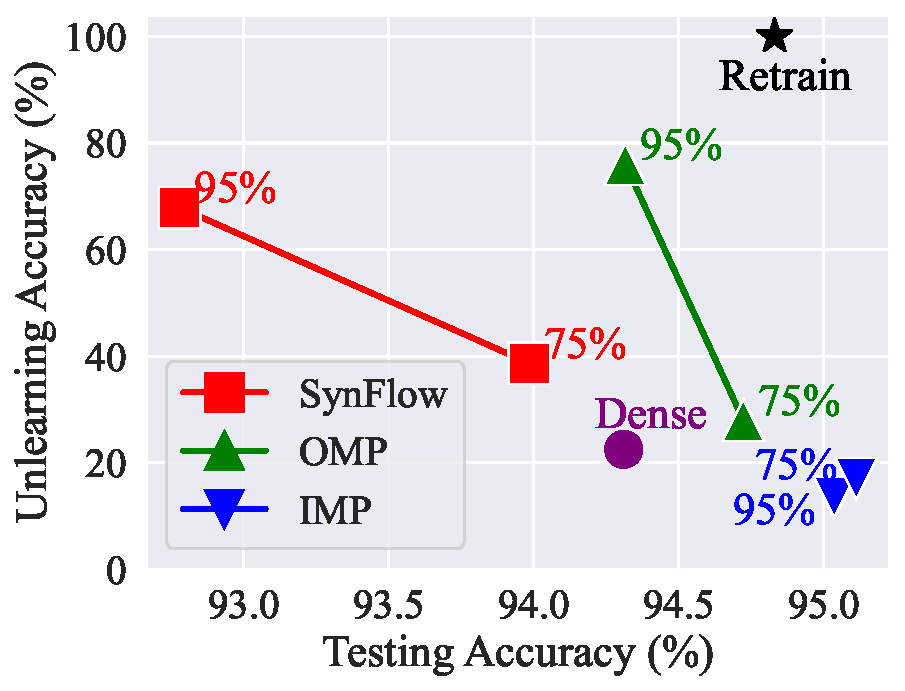
\includegraphics[width=35mm,height=!]{figs/UA_vs_pruning_retrain.pdf} &
    \hspace*{-5mm}  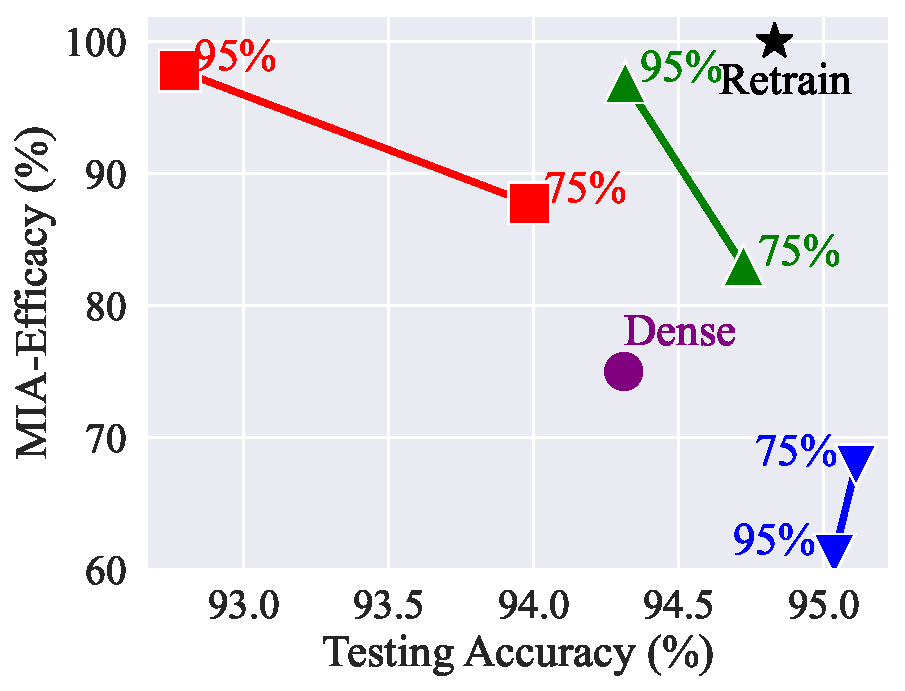
\includegraphics[width=35mm,height=!]{figs/MIA_vs_pruning.pdf} 
    \hspace*{-3mm} 
\end{tabular}}
 \vspace*{-3mm}
\caption{\footnotesize{Influence of different   pruning
methods ({\color{red}{SynFlow}}, {\color{ForestGreen}{OMP}}, and {\color{blue}{IMP}}) in unlearning efficacy ({\UA} and {\MIAF}) and generalization ({\TA})  on    (CIFAR-10, ResNet-18). \textbf{Left}: {\UA} vs. {\TA}. \textbf{Right}:   {\MIAF} vs. {\TA}. Each point is a {\FT}-based unlearned dense or sparse model (75\% or 95\% sparsity), or a retrained dense model.
%using  {\FT}. \JC{If a pruning method is proper for {\MU}, then its integration with {\FT} should  yield unlearned models with closer {\UA}, {\MIAF}, and {\TA} to {\retrain}.} 
%\JC{larger font in figs}
}}
 \vspace*{-4mm}
\label{fig: results_pruning_comparison}
\end{wrapfigure}